\documentclass{article}
\usepackage[final]{neurips}
\usepackage[framemethod=tikz]{mdframed}
\usepackage{lipsum}
\definecolor{mycolor}{rgb}{0.122, 0.435, 0.698}
\newmdenv[innerlinewidth=0.5pt, roundcorner=4pt,linecolor=mycolor,innerleftmargin=6pt,
innerrightmargin=6pt,innertopmargin=6pt,innerbottommargin=6pt]{mybox}
\usepackage[utf8]{inputenc} % allow utf-8 input
\usepackage[T1]{fontenc}    % use 8-bit T1 fonts
\usepackage[hidelinks]{hyperref}       % hyperlinks
\usepackage{url,xcolor}            % simple URL typesetting
\usepackage{booktabs}       % professional-quality tables
\usepackage{amsfonts}       % blackboard math symbols
\usepackage{nicefrac,tcolorbox}       % compact symbols for 1/2, etc.
\usepackage{amsmath}
\usepackage{enumitem}
\usepackage{microtype}      % microtypography
\usepackage{graphicx,caption}
\usepackage{xepersian}
\settextfont{XB Niloofar}
\setdigitfont{XB Niloofar}
\raggedbottom


\title{
	\vspace{-0.8em}
تمرین سری پنجم درس نظریه گروه‌ها - دکتر رضاخانی
\\
{\normalsize
\textbf{مهلت تحویل اولیه:
پنج‌شنبه ۶ اردیبهشت ماه
 سال ۱۴۰۳ تا ساعت 59:23
\\
{
\small \color{red}
به علت مشغله‌های درسی دانشجویان تا روز سه‌شنبه 11 اردیبهشت‌ماه تمدید شد.
}
\\
\vspace{-0.4em}
از طریق سامانه
\href{https://cw.sharif.edu/}{درس‌افزار شریف}
}
}
\vspace{-0.6em}
}

\usepackage[utf8]{inputenc}

\usepackage[english]{babel}
\setlength{\parindent}{3.5em}
\setlength{\parskip}{0.5em}
\renewcommand{\baselinestretch}{1.0}

\usepackage{calrsfs}
\DeclareMathAlphabet{\pazocal}{OMS}{zplm}{m}{n}
\newcommand{\La}{\mathcal{L}}
\newcommand{\Lb}{\pazocal{L}}

\newtcolorbox{boxes}[3][]
{
	before upper=\renewcommand\thempfootnote{\fnsymbol{mpfootnote}},
	colframe = #2!25,
	colback  = #2!10,
	coltitle = #2!40!black,  
	title    = {\textbf{#3}},
	#1,
}

\newenvironment{exercise}[3][\unskip]{%
	\par
	\noindent
	\textbf{تمرین
		#1
		[#2 امتیاز] 
		\def\temp{#3}\ifx\temp\empty
		: 
		\else
		: #3 \vspace{0.5em} \\ \noindent
		\fi
}}{}

\author{
حسین محمدی\\
  \lr{
  		\href{mailto:hossein.mohammadi.imp@gmail.com}{\texttt{	hossein.mohammadi.imp@gmail.com}}} \\
  \And
  زهرا کبیری\\
 \lr{
  		\href{mailto:kabiri.zahra98@gmail.com}{ \texttt{kabiri.zahra98@gmail.com}}}\\
  }

\begin{document}


\begin{minipage}{0.1\textwidth}% adapt widths of minipages to your needs
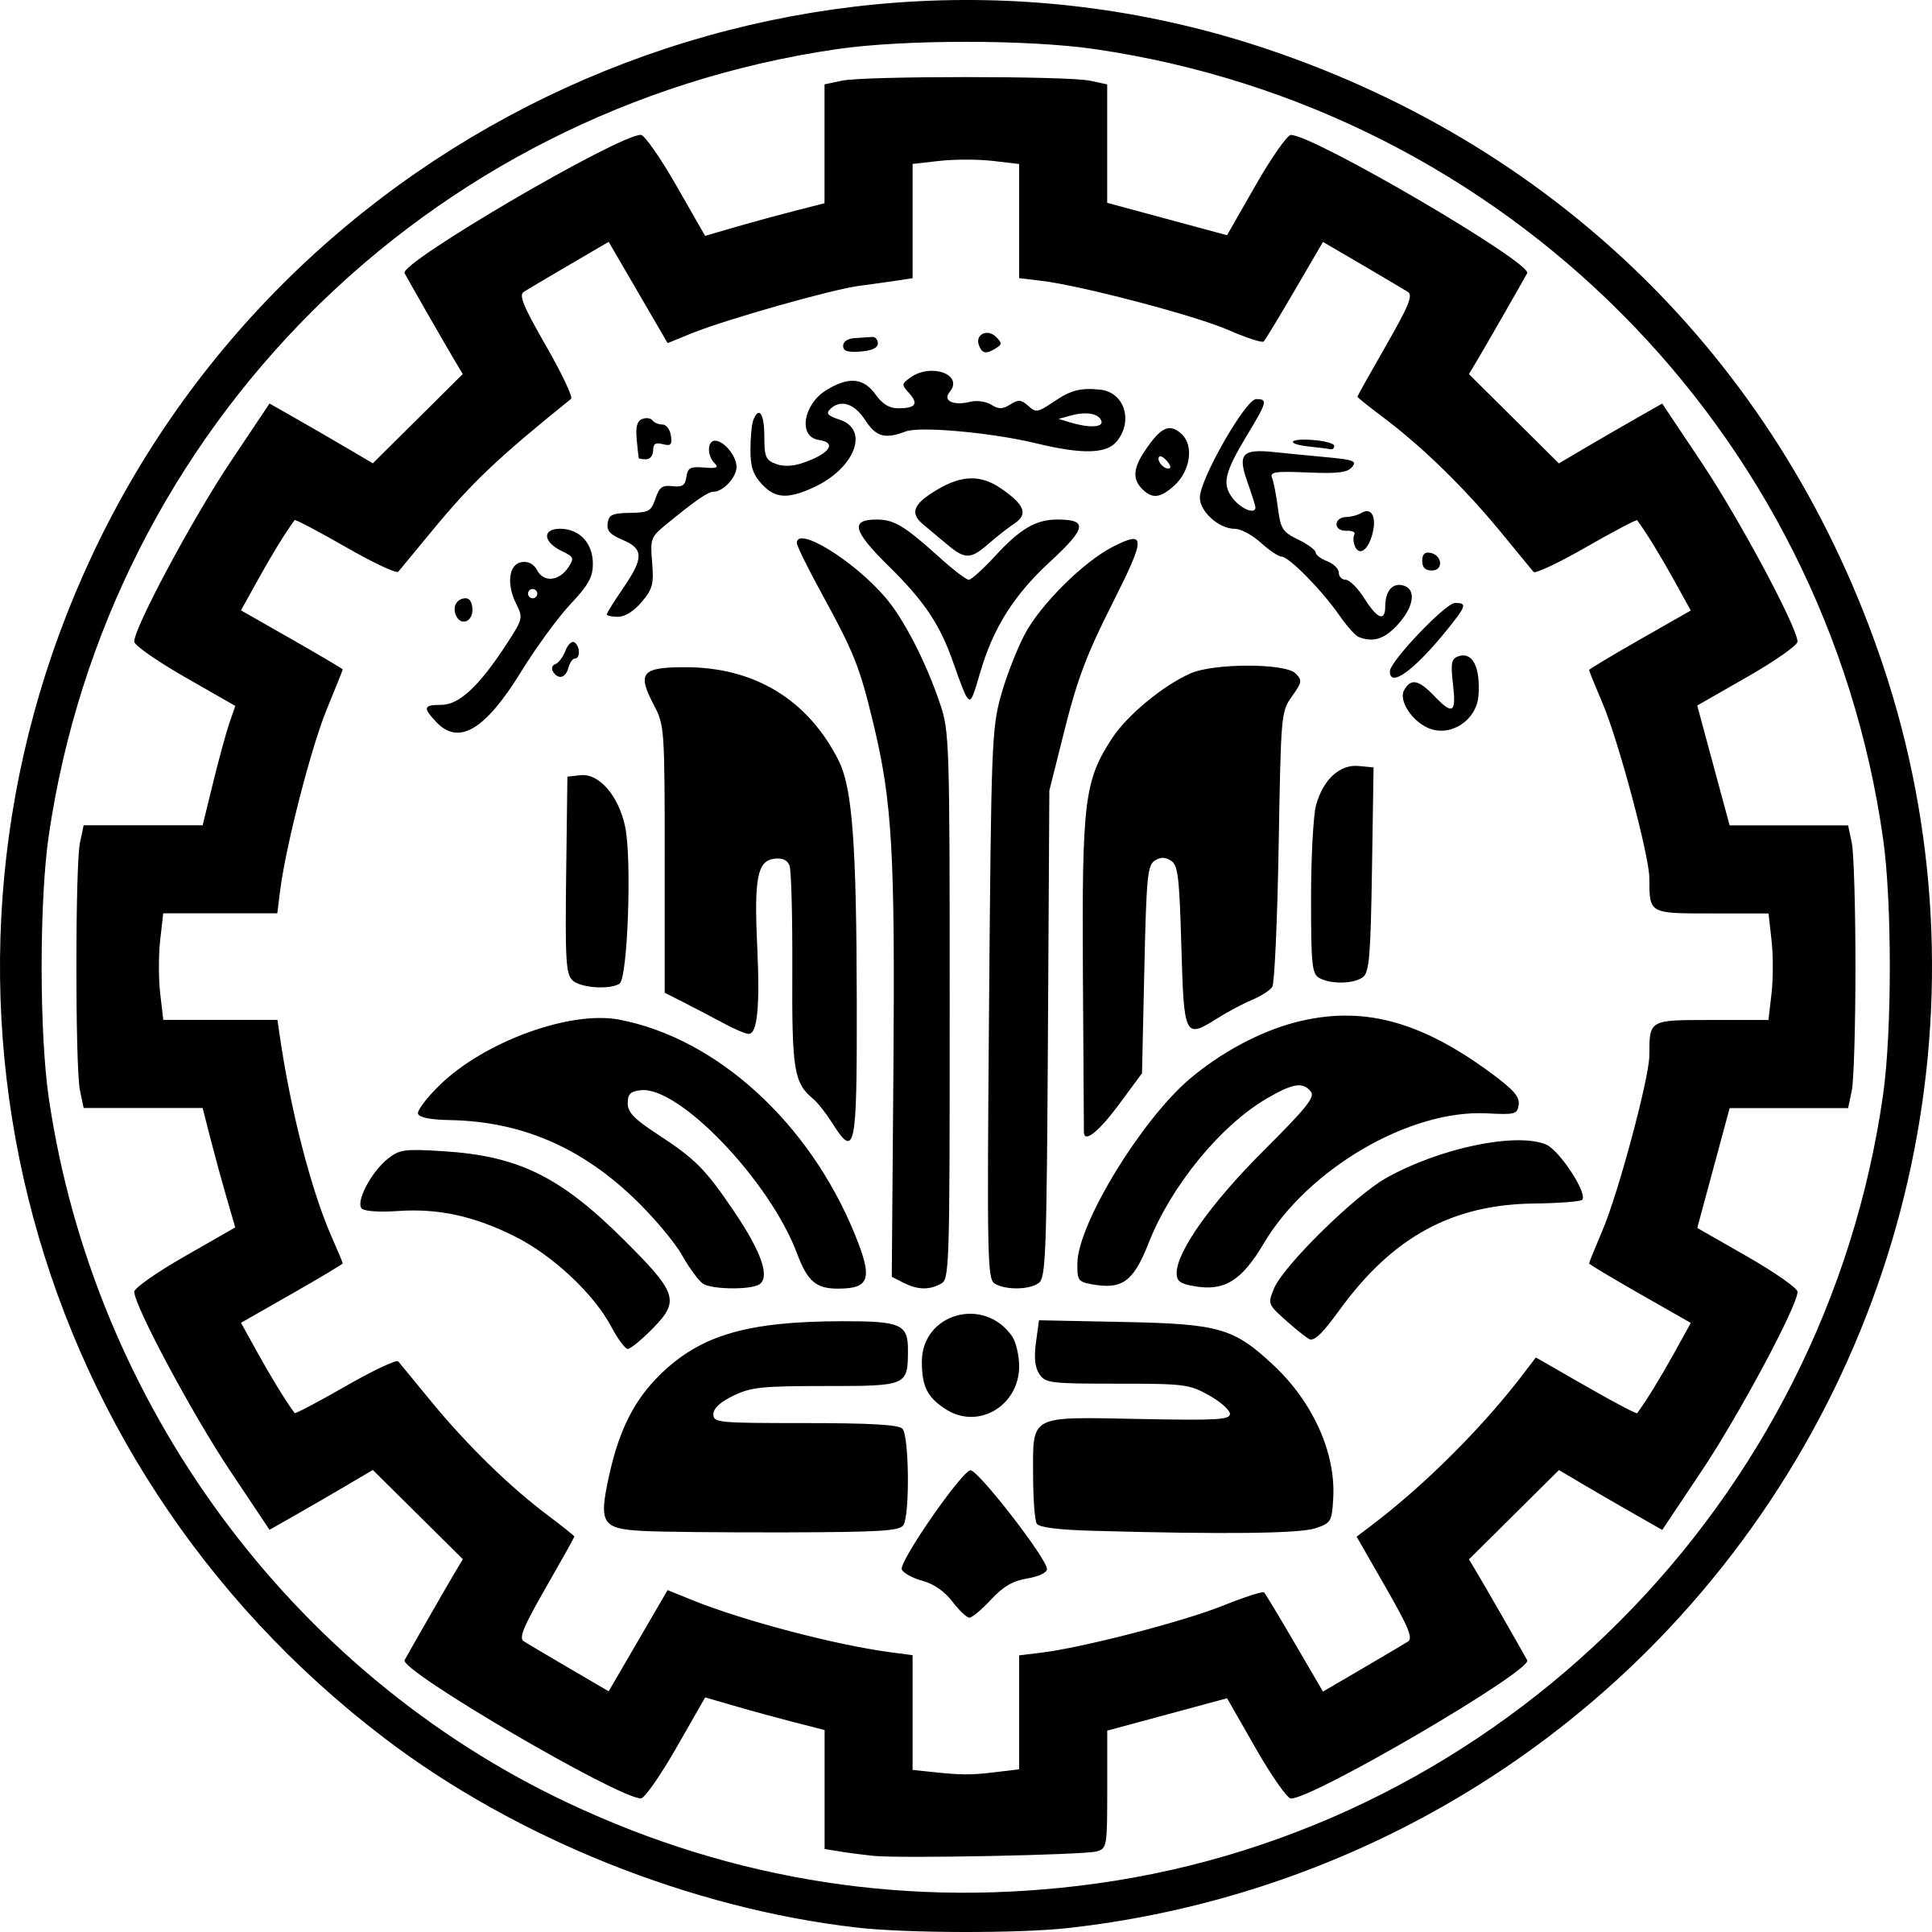
\includegraphics[width=1.1cm]{sharif-logo.png}
\end{minipage}%
\hfill%
\begin{minipage}{0.9\textwidth}\raggedleft
دانشگاه صنعتی شریف\\
زمستان ۱۴۰۲ - بهار ۱۴۰۳\\
\end{minipage}

\makepertitle

\begin{boxes}{black}{تعاریف}
	با اثر گروه روی مجموعه‌ها آشنا شدید. اینجا با هم یک سری تعاریف را مرور می‌کنیم؛ تعاریفی که احتمالا در درس هم خواهید دید. اول فرض کنید گروه $G$، از چپ روی مجموعه‌ی $S$ اثر کند
	\footnote{مشابها این مفاهیم را برای اثر از راست هم می‌توانید تعریف کنید.}
	. 
	
	\textbf{پایدارساز
	\LTRfootnote{Stabilizer}:
	}
	برای هر عضو $s\in S$ مجموعه‌ی پایدارساز این عضو را به شکل زیر تعریف می‌کنیم
	\[
	\text{Stab}_g(s) = \{g\in G \; \big| \; g.s=s\}
	\]
	یا به طور کلی‌تر، برای هر زیرمجموعه‌ی $T$ از مجموعه‌ی $S$، می‌توانیم تعریف کنیم
	\[
	\text{\lr{Fix}}_G(T) = \{g \in G \;\big|\; g.x = x \;\; \text{\lr{for all}}\; x \in T\}
	\]
	همانطور که از اسمشان هم پیداست، اعضای پایدارساز  یک عضو خاص از مجموعه را ثابت نگه می‌دارند.
	
	\textbf{مدار
	\LTRfootnote{Orbit}
	:}
	 عنصر 
	$s\in S$ را 
	معین کنید؛ مدار $s$ تحت اثر گروه 
	$G$ به شکل زیر تعریف می‌شود
	\footnote{از آقای محمد قوهستانی و خانم مژده محمودیان برای تذکرشان ممنونیم.}
	\[
	\text{\lr{Orb}}_G(s) = \{ g.s \; \big| \; g \in G\}
	\]
	
	با این تعاریف، می‌توانید به دسته‌های تزویجی با کمک «اثر گروه روی خودش»، از منظری جدید نگاه کنید. هر گروه $G$ به شکل زیر روی خودش اثر می‌کند:
	\[
	 g\in G , s \in G \quad,\quad g.s = gsg^{-1}
	\]
	آن‌وقت کلاس‌های تزویجی چیزی جز مدار این اثر نیستند.

\end{boxes}

\begin{exercise}[21]{25}{}
	میدان 
	$\mathbb{F}_p$
	، که در آن $p$ عددی اول است، درنظر بگیرید. گروه 
	$G = \text{GL}_n(\mathbb{F}_p)$
	را گروه متشکل از ماتریس‌های وارون‌پذیر
	$n \times n$
	با درایه‌های عضو میدان 
	$\mathbb{F}_p$
	فرض کنید. 
	
	\noindent
	می‌دانیم که اعضای این گروه با ضرب ماتریسی روی فضای برداری 
	$\mathbb{F}_p^n$
	، یعنی فضای برداری $n$-بعدی با ضرایب از میدان 
	$\mathbb{F}_p$
	اثر می‌کنند. حالا بردار 
	$e_1$ 
	از این فضای برداری را به شکل زیر بگیرید
	\footnote{از آقای ارمیا هلالی برای تذکر اشتباه تایپی ممنونیم.}
	:
	\[
	e_1 = (1,\underbrace{0,\dots,0}_{\text{\lr{n-1} بار}})
	\]
	مدار این عضو را (تحت اثر گروه $G$) پیدا کنید و اعضایش را بشمارید. همچنین مرتبه‌ی 
	$\text{Stab}_G(e_1)$
	را هم پیدا کنید.
	
\end{exercise}
\newpage
\begin{exercise}[22]{35}{قضیه مدار-پایدار‌ساز }
	فرض کنید گروه متناهی $G$، از چپ روی مجموعه‌ی $S$ اثر کند. نشان دهید که برای هر 
	$s \in S$
	 داریم:
	 \begin{equation*}
	 	\begin{aligned}
	 		|G| = |\text{\lr{Orb}}_G (s)|. |\text{\lr{Stab}}_G(s)|.
	 	\end{aligned}
	 \end{equation*}
	
\end{exercise}
\begin{boxes}{black}{یادآوری تعریف بهنجارساز و پایدارساز}
	بهنجارساز یک زیرمجموعه از گروه، مجموعه‌ی تمام اعضایی از گروه است که شرط بهنجاری را با تمام اعضای زیرمجموعه دارد.
	\[
	N_G(S) = \{g\in G \;\big| \; gsg^{-1} \in S, \; \forall s\in S\}
	\]
	همچنین؛ مرکزساز یک مجموعه، مجموعه‌ی تمامی اعضایی از گروه است که با تمامی اعضای زیرمجموعه‌ی مذکور جابه‌جا می‌شوند.
	\begin{equation*}
		\begin{aligned}
			C_G(S) = \{
			g \in G \; \big| \; gs=sg , \; \forall s\in S
			\}
		\end{aligned}
	\end{equation*}
\end{boxes}
\begin{exercise}[23]{15}{ }
	اگر 
	$H$ زیرگروهی مرتبه دو از گروه $G$ باشد، نشان دهید که 
	$C_G(H) = N_G(H)$.
\end{exercise}
\begin{exercise}[24]{25}{ }
کلاس‌های تزویجی گروه 
$D_5$ را به‌دست آورید.
\end{exercise}
\vspace{1em}

\begin{boxes}{green}{پیشنهاد مطالب برای مطالعه بیشتر}
	از قضایای بسیار مهمی که خوب هست بدانیم؛ معادله کلاس
	\LTRfootnote{Class equation}
	است. وقتی گروه $G$ مطابق جعبه‌ی «تعریف» روی خودش اثر می‌کند:
	\[
	|G| = |Z(G)| + \sum_{s \in \text{\lr{\tiny disjoint nontrivial orbits}}} \frac{|G|}{|\text{\lr{Stab}}_G(s)|}
	\]
	در مسائل مربوط به رنگ‌آمیزی گرافها و ترکیبیات، معادله کلاس بسیار راهگشاست. احتمالا در این موارد حرف نزنم و سوالی هم حل نکنم؛ اما با یک جستجوی ساده می‌تواند این مسائل را پیدا کنید و راه‌حلشان را ببینید.
	
	همچنین استفاده از قضایایی که در تمرین دیدید، چارچوب خوبی را برای فهم و استفاده از قضایای سیلو فراهم می‌کند.
\end{boxes}
 \end{document}
